% !TEX TS-program = XeLaTeX
% !TEX encoding = UTF-8 Unicode

\chapter{绪论}
\label{chap00}

\section{选题的背景与意义}
随着社会的发展,人类的生产和生活对能源的需求越来越大。在积极开发新能源的同时,
必须看到,当前,尤其是我国对传统化石能源的依赖仍然非常大,特别是煤炭。
更加规范的管理煤炭的生产、运输、使用等在对于安全生产、保护环境等是非常重要的。
其中,煤仓是煤炭的生产、运输、使用等环节中都非常重要的设施,其可以作为各环节
之间的缓冲,也可以避免煤炭露天堆放产生的消耗和环境污染,因此在煤矿、煤炭销售、
热电厂、煤化工厂等中都得到了广泛的使用。

作为一种大型的工业建筑,其直径甚至可以达到百余米,高可达数十米,装载能力可以
达到数十万吨。如此巨大的建筑、如此多的载荷将是对设计、施工和运营的巨大考验,
也是对地基和煤仓壁的巨大考验。

对于此类大型建筑进行变形监测是非常重要,也是非常必要的。历史上,曾经有很多的教训\ucite{DEFORM03}\ucite{HSX-PHD}:
\begin{asparaitem}[$\bullet$]
\item 法国67米高的马尔巴塞(Malpasset)拱坝1959年垮坝
\item 意大利262米高的瓦依昂(Vajoint)拱坝1963年因库岸大滑坡导致涌浪翻坝且水库淤满失效
\item 美国93米高的提堂土坝1976年溃决
\item 我国板桥和石漫滩两座土坝1975年洪水漫坝失事
\end{asparaitem}
当然也有非常多因为得力的监测工作避免或者降低生命财产损失的案例\ucite{DEFORM03}\ucite{HSX-PHD}:
\begin{asparaitem}[$\bullet$]
\item 1985年6月12日长江三峡新滩大滑坡的成功预报成功确保灾害损失减少到了最低限度
\item 隔河岩大坝外观变形GPS自动化监测系统在1998年长江流域抗洪错峰中所发挥的巨大作用,确保和安全渡汛,避免了荆江大堤灾难性的分洪
\end{asparaitem}

安全监测除了及时掌握建筑物的工作性态,确保其安全外,还有多方面的必要性。
美国垦务局认为,
对建筑物及地基进行长期和系统的监测,是诊断、预测、法律和研究等四个方面的需要\ucite{DEFORM03}\ucite{HSX-PHD}:
\begin{asparaitem}[$\bullet$]
\item 诊断的需要。包括验证设计参数与改进设计,对新施工技术的优越性进行评价;
对不安全迹象和险情进行诊断并采取措施予以加固;以及验证建筑物运行是否处于持续正常状态。
\item 预测的需要。利用长期积累的观测资料掌握变化规律,对建筑物的未来性态做出及时有效的预报。
\item 法律的需要。对由于工程事故而引起的责任和赔偿问题,观测资料有助于确定其原因和责任,以便法庭做出公正判决。
\item 研究的需要。观测资料是建筑物工作性态的真实反映,为未来设计提供定量信息,
可改进施工技术,利于设计概念的更新和对破坏机理的了解。
\end{asparaitem}

煤仓、大坝等工业建筑与其它民用建筑相比,有其特殊的地方,包括:
\begin{asparaitem}[$\bullet$]
\item 建设阶段相比运营阶段所受的压力要小很多,这样,其它一些建筑在建设时就会表现出来的问题,
对于这些建筑可能要到运营一段时间之后才能表现出来。
\item 运营阶段受压力变化会很大,比如,水库可能干涸,煤仓可能出现空仓,
这种变化是否会对建筑的稳定产生巨大影响需要特别关注,也会对数据的处理提出更高的要求。
\end{asparaitem}

\section{现有的观测手段和数据处理方法}
施工和运营阶段对于建筑物进行变形监测是非常重要和必要的。
为了解决这些问题,这个更好地对建筑物的形变进行观测和预报,掌握建筑物形变的规律,
人们采取了非常多的措施来观测,引入了许多的数据处理方法。

\subsection{建筑物变形监测的方法}
随着技术的发展,尤其是通信、传感器等技术的发展,
变形监测领域引入了很多新的测量手段。
未来,随着技术的继续发展,还会有更多的新测量手段引入。
张正禄等总结了现有的变形监测的技术手段\ucite{DEFOR07}。
\subsubsection*{常规大地测量方法}
常规大地测量方法就是利用常规大地测量仪器和方法,
包括经纬仪,水准仪、电磁波测距仪、全站仪以及GNSS接收机等,
测量方向、角度、边长、高差等量,可以布设成网形来确定坐标的网平差法、
交会法、极坐标法、卫星定位法,以及几何水准、三角高程法等。
\subsubsection*{摄影测量方法}
与其它方法相比,摄影测量方法有着可以不接触被测变形体,
可快速获取变形体上的任意点并快速获取变形过程,
信息量大、利用率高、后处理方法多等优点,
在适合使用摄影测量的变形监测领域得到的广泛的使用。
近年来发展的数字摄影测量和实时摄影测量将有更好的应用前景。

摄影测量方法的精度\ucite{LIZHONG-CAMEAR}\ucite{SHEN-QINGXIONG-CAMEAR}\ucite{GU-GAO-QIU-CAMEAR}
\ucite{LU-HUANG-LI-CAMEAR}\ucite{RTP-CAMEAR}
主要取决于像点坐标的测量精度和摄影测量的几何强度。
前者与摄影机和量测仪的质量、摄影材料质量有关,后者与摄影站和变形体之间的关系
以及变形体上控制点的数量和分布有关。
目前相片坐标精度可达2~4${\mu}$m,目标点精度
可达摄影距离的${1/10^5}$。
\subsubsection*{短距离测量的方法}
由于电磁波测距有着其固定的系统误差,因此在测量较小的距离(小于$50m$时)不宜采用这种方法。
实际生产中经常使用的是机械法,如Gerick金属丝测长仪:将很细的金属丝在
固定拉力下绕在因瓦测鼓上。机械法的优点是受温度影响小,在此测程下精度可以优于$1mm$。
\subsubsection*{准直法和铅直法}
准直测量就是要测量观测点偏离基准线(或基准面)的垂直距离的过程,可以包括水平准直和铅直两种。
水平准直测量也经常被直接称为准直测量。
偏离基准线或基准面的距离值称为偏距(或垂距),测量偏距的方法同样有光学法、光电法和机械法等。
铅垂线可以用光学法、光电法或机械法产生。铅直法中的机械法主要是可以克服风和摆动的影响,
最常用的机械法是正、倒垂线法。\ucite{LIU-WU-LEVEL}
\subsubsection*{液体静力水准法}
基于贝努利方程,即对于连通管中处于静止状态的液体压力,满足$P+{\rho}gh=C$,
其中$P$为空气压力,$\rho$为液体密度,$g$为重力加速度,$h$为液体水柱高,$C$为一常数。
利用这个原理制成了液体静力水准测量仪,可用于观测多点之间的高差,精度也非常高。
因为此方法不要求通视,故非常适合建筑物内部的沉降观测,尤其是使用常规光学水准法观测较困难且高差又不太大的情况;
正因为液体静力水准测量的这些优点,其在粒子加速器等大科学装置上得到了广泛使用。\ucite{BJ-ELEC}\ucite{SH-HLS}
若一个观测头安装在基准点上,其它观测头安装在目标点上,进行多期观测,则可获取多个目标点的垂直位移。
液体静力水准测量系统的另外一个巨大的优势是可以非常方便的将液面变化转换成电感信号,而便于采用自动读数装置,
可实现持续监测,监测点可达上百个。\ucite{HE-XIAOYE-STATIC}
此外还发展了移动式系统,克服了不便于移动的缺点,观测的高差可达数米,
因此也可用于桥梁的沉降变形监测。\ucite{LINQIN-STATIC}
\subsubsection*{挠度测量}
挠度曲线为相对于水平线或铅垂线(称基准线)的弯曲线,在曲线上某点到基准线的距离称为挠度。
大坝的挠度曲线及其随时间的变化可以通过正、倒垂线法或倾斜测量方法获得。
房屋类高层建筑物的挠度可以由观测不同高度处的倾斜来换算求得。
大桥的挠度则可以使用GPS、全站仪、摄影测量等方法测得。\ucite{DAQ-ND}
\subsubsection*{倾斜观测}
两点之间的倾斜可以使用测斜仪直接测得。测斜仪包括摆式测斜仪、
伺服加速度计式测斜仪以及电子水准器等。采用电子测斜仪可进行动态观测。
两点之间的倾斜也可以用测量高差或水平位移,通过两点间距离间接获得。
\subsubsection*{裂缝的观测方法}
工程建筑物的裂缝观测内容包括对裂缝编号,观测裂缝的位置、走向、长度、宽度等。
对于重要的裂缝,要埋设观测标志,用游标卡尺定期地测定两个标志头之间距离的变化,
确定裂缝的发展情况。
对于建筑预留缝和岩石缝隙这种更小距离的测量,一般通过预埋内部测微计和外部测微计进行。
测微计通常由金属丝或因瓦丝与测表构成,其精度可优于$1mm$。\ucite{HUADONG-CEWEI}
\subsubsection*{振动的观测方法}
对于塔式建筑物,在温度和风力荷载作用下会来回摆动,从而就需要对建筑物进行动态观测,
即振动(摆动)观测。有的桥梁也需要进行振动观测,对于特高的房屋建筑,也存在振动现象。
观测建筑物的振动,可采用专门的光电观测系统,其原理与激光铅直相似,也可以采用GNSS
技术做持续的动态振动观测。\ucite{ZHD-SEN}
\subsubsection*{三维激光扫描测量法}
三维激光扫描仪在不同位置对被测对象进行扫描得到“点云”,通过后处理软件可获取物体
在给定的坐标系下的三维坐标。车载、机载激光扫描仪将成为21世纪地面数据采集的
主要手段,已经被广泛应用在工程建筑和变形监测方面,并将成为一种广泛应用的、
重要的变形监测方法。\ucite{HUWHH-SCANNER}\ucite{XUWANG-SCANNER}
\subsubsection*{变形监测的自动化}
变形监测的自动化要求基于下述原因:
\begin{asparaitem}[$\bullet$]
\item 变形速度太快
\item 监测点太多——需要同一时刻获得许多个测点上的变形;
\item 监测间隔太短——变形过程需要大量短时间间隔的观测数据描述;
\item 监测环境太恶劣——噪声、高压、高热、高磁场或人无法到达;
\item 监测不能影响生产和运行管理。
\end{asparaitem}
基于信号转换的传感技术,可以把变形监测中需要确定的距离、角度、高差、倾角等几何量
及其微小变化转化为点信号。将这些用于变形监测以及精密测量的传感器安装在伸缩仪、
应变仪、准直仪、铅直仪、测斜仪以及经历水准测量系统中,通过数据获取、信号处理、
数据转换与通信,可将成百上千个测点上的监测数据传送到数据终端或数据处理中心,
实现变形的持续监测、数据的自动记录、传输与处理。\ucite{GUIZHCH-GEOROBOT}
\ucite{HANLI-LEVELBOT}\ucite{FENG-LI-TRANS}

\subsection{变形分析方法}
变形分析研究主要涉及变形的数据分析、物理解释以及预报等很多方面,其通常被分为几何分析和物理解释两部分。
变形的几何分析就是要描述变形体形状及大小的变化,其任务为描述变形的时空特性。
变形物理解释是要解释变形的原因。\ucite{DEFORM03}\ucite{HSX-PHD}

\subsubsection*{1) 传统变形的时空特征分析及其建模方法}
传统的变形几何分析主要包括参考点的稳定性分析、观测值的平差处理和质量评定以及变形模型参数估计等内容。
\paragraph*{参考点的稳定性分析} 
参考点或一定基准是监测变形信息的基础,如果选择了不稳定或不统一的基准,
获取到的变形值反映的就不是正确的变形值。变形基准的稳定性和正确性是变形监测数据处理首先必须考虑的问题。
过去的研究给出了很多对周期性监测网参考点的稳定性分析的方法,
例如,A. Chrzanowski论述的这样的5种方法\ucite{Chrzanowski-compare}:
\begin{asparaitem}[$\bullet$]
\item 以方差分析进行整体检验为基础的的Hannover法,即“平均间隙法”
\item 以$B$检验法为基础的Delft法,即单点位移分量法
\item 以方差分析和点的位移想了为基础的Karlsruhe法
\item 考虑大地基准的Munich法
\item 以位移的不变函数分析为基础的Fredericton法
\end{asparaitem}
后来又发展出了稳健-$S$法,也被称为逐次定权迭代法。\ucite{CJS:CJS473}
\paragraph*{观测值的平差处理和质量评定}
变形值的精度和可靠性受到观测值的质量好坏的直接影响。
该方面主要牵涉到平差基准、观测值质量、粗差处理、变形的可区分性等几项内容。
在固定基准的经典平差基础上,发展了重心基准的自由网平差和拟稳基准的拟稳平差\ucite{ZHOUJW-Outlier}。
在W. Baarda提出数据探测法\ucite{BAARDA-DETECT}后,
粗差探测与变形的可区分性研究成果已经极为丰富,这以体现在李德仁\ucite{LIDEREN-Outlier}、
黄幼才\ucite{HYOUC-Outlier}、陶本藻\ucite{TAO-Outlier}等的著作中。
\paragraph*{变形模型参数估计}
陈永奇\ucite{CHYQ-OBV}概括了两种基本的分析方法,即直接法和位移法。直接法是利用原始的重复观测值
之差计算应变分量或它们的变化率;位移法是利用各观测点坐标的平差值之差(位移值)计算应变分量。
同时他还提出了变形分析通用法,研制了相应的软件DEFNAN。

\subsubsection*{2) 动态变形分析}
从20世纪70年代末至90年代初,对几何变形分析研究得较为完善的是用常规地面测量
技术进行周期性监测的静态模型,但它考虑的仅仅是变形体在不同观测时刻的空间状态,并没有
很好的建立各个状态之间的联系,更谈不上变形监测自动化系统的变形分析研究。事实上,
变形体在不同状态之间是具有时间关联性的。为此,后来许多学者转向了对时序观测数据的
动态模型研究,如变形的时间序列分析方法建模;基于数字信号处理的数字滤波技术分离时效分量;
变形的卡尔曼滤波模型;
用FIR(Finite Impulse Response)滤波器抑制GPS多路径效应等\ucite{2002287011810}。
\paragraph*{频谱分析方法}
动态变形分析既可以在时间域进行,也可以在频率域进行。频谱分析方法是将时域内的数据序列
通过傅立叶级数转换到频域内进行分析,有利于确定时间序列的准确周期并判别隐蔽性和复杂性的
周期数据。频谱分析法的苛刻条件是数据序列的等时间间隔要求,这为一些工程变形检测分析的
实用性增加了难度,因为对于非等间隔序列进行插补和平滑处理必然会带入人为因素的影响。

多年来,对变形数据分析方法研究是极为活跃的,除了传统的\textbf{多元线性回归法}以及
上述的\textbf{时间序列分析法}、\textbf{频谱分析法}和\textbf{滤波技术}之外,
\textbf{灰色系统理论}、\textbf{神经网络}等非线性时间序列预测方法也得到了一定的应用。
比如,应用\textbf{灰关联分析方法}研究多个因变量与多个自变量的变形问题\ucite{YINHUI-GREY};
应用\textbf{灰色理论}建模预测深基坑事故隐患;
应用\textbf{人工神经网络建模}进行短期的变形预测\ucite{MAWANG-BP}。
其它非线性科学理论也在变形研究中得到了反映。
例如根据突变理论,用尖点突变模型研究大坝及基岩的稳定性\ucite{XUEZHANG-MUTATION};
将大坝运行性态堪称一种非线性动力系统,来研究大坝观察数据序列中的混沌现象\ucite{WANGLIU-CHAO}。

在线实时分析与监控的方法对于进行即时预报与监控、在紧急关头为突发性灾害提供即时决策咨询。
已有研究表明,采用递推算法的贝叶斯动态预测模型进行大坝监测的动态分析是可行的\ucite{BAYESIAN-DAM}。
在隔河岩大坝GPS自动化监测系统中,采用递推式卡尔曼滤波模型进行全自动卡尔曼滤波进行全自动
在线实时数据处理起到了较好效果\ucite{GEHEYAN}。

在变形分析中,人们研究了多种方法的结合以弥补单一方法的缺陷。
例如,灰关联聚类分析法,即模糊数学原理与灰色理论相结合 —— 进行多测点建模预测;
应用模糊人工神经网络方法 —— 模糊数学与人工神经网络相结合 —— 建模进行边坡和大坝的变形预报;
在回归分析中,提出了应用抗差估计理论对多元回归分析模型进行改进的抗差多元回归模型来处理数据序列的粗差问题;
还有研究认为,要解决大坝安全监控专家系统开发中“瓶颈”问题可以使用人工神经网络与专家系统相结合的思路。\ucite{DEFORM03}

\textbf{小波分析理论}诞生于20世纪80年代末的小波分析理论,是一种新的时频局部化分析方法,
被认为是自傅立叶分析方法后的突破性进展。应用小波方法,进行时频分析,可望有效地求解
变形的非线性问题,通过小波变化提取变形特征。小波分析为高精度变形特征提取提供了一种
数学工具,可实现其它方法无法解决的难题,
对非平稳信号消噪有着其它方法不可比拟的优点\ucite{DENOISING-WAVELET}。

\subsubsection*{3) 变形物理解释的进展}
变形物理解释的方法可分为统计分析法、确定函数法和混合模型法三类。

\textbf{统计分析法}以回归分析模型为主,具有后验的性质
其方法是根据分析得到的所观测的变形与外因的相关关系建立载荷-变形之间的数学模型。
回归分析模型包括多元回归分析模型、逐步回归分析模型、主成分回归分析模型、模糊聚类分析和岭回归分析模型。
回归分析模型的发展包括时间序列分析模型、灰关联分析模型、模糊聚类分析模型以及动态响应分析模型等。

\textbf{确定函数法}以有限元法为主,即在一定的假设条件下,利用变形体的物理、力学性质,
建立应力与应变之间的函数模型,再使用这种方法得到的函数模型预报在某种大小的载荷作用下变形体可能的变形。
这种模型具有“先验”的性质,物理概念比统计模型更明确,但缺点是往往计算工作量较大,
对基本资料的要求也较高。

\textbf{混合模型}是将有限元法应用于效应量关系比较明确的原因量,
而将统计模型应用于另一些与效应量关系不很明确或采用相应的物理理论计算成果难以确定它们之间函数关系的原因量,
然后与实际值进行拟合。

\textbf{反分析}即效仿系统识别理论,依据正分析成果,通过一定的理论分析,
借以反求建筑物及其周围的材料参数,并以此来寻求某些规律和信息,及时反馈到设计、施工和运行中去。
反分析按其实际内涵包含既有联系又有区别的反演分析和反馈分析。

由于变形的物理解释涉及到多学科的知识,已远不是测量人员所能够独立完成的,
所以需要相关学科专家的共同合作。

\subsubsection*{4) 变形分析研究的发展趋势}
近年来,变形分析进行了大量实践并取得了大量研究成果,其发展趋势可能将要体现在如下几个方面\ucite{DEFORM03}:
\begin{asparaitem}[$\bullet$]
\item 数据处理和分析将向自动化、智能化、系统化、网络化和实时化方向发展,时空模型
和时频分析受到更大的重视,数字信号处理技术的应用范围将更加广泛。
\item 会加强对各种方法和模型的实用性研究,变形监测系统软件的开发不会局限于某一个固定模式,
随着变形监测技术的发展,变形分析新方法的研究将会不断涌现。
\item 由于变形体变形的不确定性和错综复杂性,对它的进一步研究呼唤着新的思维方式和方法。
由系统论、控制论、信息论、耗散结构论、相同学、突变论、分形与混沌动力学等所构成的系统科学
和非线性科学在变形分析中的应用研究将得到加强。
\item 几何变形分析和物理解释的综合应用将深入发展,以知识库、方法库、数据库和多媒体库为主体
的安全监测专家系统的建立是未来发展的方向,变形的非线性系统问题将是一个长期研究的课题。
\end{asparaitem}


\section{煤矿与煤仓}
\subsection{煤矿}
煤矿是富含煤炭资源的地方,通常也指采用地下采掘或露天采掘方式生产煤炭的工厂。

当矿层接近地表时,使用露天开采的方式较为经济。矿层上方的土称为表土。
在尚未开发的表土带中埋设炸药,接着使用挖泥机、挖土机、卡车等设备移除表土。
这些表土则被填入之前已开采的矿坑中。表土移除后,矿层将会暴露出来;
这时将矿块钻碎或炸碎,使用卡车将矿砂运往选煤厂做进一步处理。
当矿石开采完毕,在隔壁重复同样的步骤。

露天开采的方式可比地下开采的方式获得较大比率的煤矿,因为较多的矿层被利用。
露天开采煤矿可以覆盖数平方公里的面积。世界约$40\%$的煤矿生产使用露天开采方式。

当大部份矿层均远离地表时,无法使用露天开采的方式,必须要采用地下开采的方式。
地下开采目前占世界煤矿生产的$60\%$。
在矿坑,通常使用房柱法在矿层中推进,梁柱用来支持矿坑。
通常有四种方法从地下开采煤炭:长壁开采、连续开采、爆破开采和短壁开采。

煤矿在超过50个国家中商业开采。煤炭目前在中国是最重要的能源,
2005年中国约有$80\%$的能源来自于燃煤。

\subsection{煤仓的特点}
煤仓是煤矿中重要的基础设施,有球形煤仓、筒形煤仓等。
其中筒形煤仓是煤仓的传统形式,也是现在的主流形式。

筒仓主要用于粮食水泥、煤炭等行业的储料容器。\ucite{BULKER-WALL}
常用工业筒仓一般是指贮存粒状或粒状松散的石膏粉、面粉、水泥等的立式容器。
平面形状一般为网形,个别因为场地和工艺要求而做成矩形。
根据高度和平面尺寸及受力特点,筒仓可分为浅仓和深仓两类。

其中深仓容量大、占地少,不污染环境。
尤其圆形深仓受力合理,也比较经济,因此使用得越来越广泛。

筒仓荷载包括永久荷载和可变荷载两部分。
永久荷载包括:结构自重、填料、设备自重等;
可变衙载包括贮料荷载、楼面及屋面活荷载、风荷载、雪荷载等。
永久荷载的倚载分项系数:其效应对结构不利时取1.2;
其效应对结构有利时取1.2。可变荷载的荷载分项系数:贮料荷载1.3;
其它荷载1.4。为计算方便,贮料荷载的计算一律按满仓计算。
贮料荷载对仓壁的压力标准值,根据浅仓和深仓受力特性,计算方法不同。
\begin{figure}[!htbp]
   \centering
   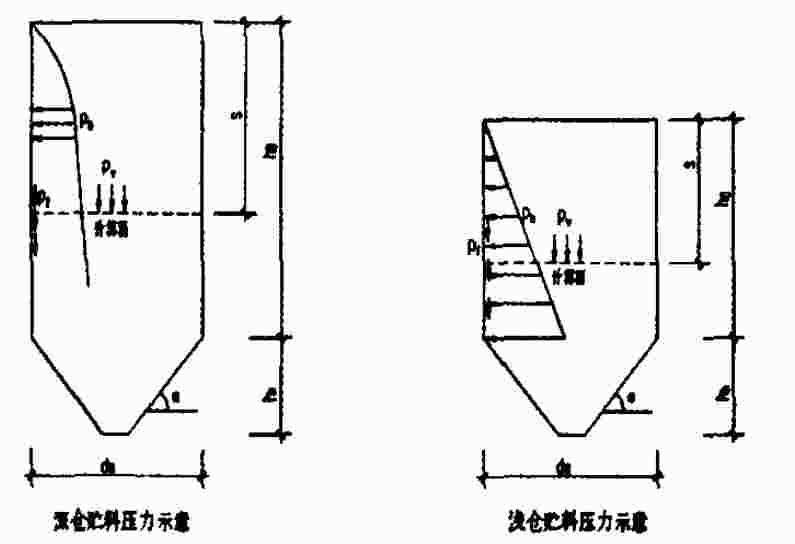
\includegraphics[scale=0.5]{bulker-carve.jpeg}
   \bicaption[figure:bulker-carve]{煤仓结构示意图}{煤仓结构示意图}
		{Fig.}{Schematic diagram of Coal bulker}
\end{figure}

\subsubsection*{煤仓的一般结构}
1) 圆形筒仓仓壁厚度$t$一般为:
\begin{equation}
t=\frac{d_n}{100}+100
\end{equation}
其中,$d_n$为筒仓的直径。
最小厚度不小于$100mm$,当直径大于15m的筒仓,壁厚不小于$300mm$。

2) 筒仓的混凝土强度等级不低于C25,
	露天冻融环境条件下混凝土强度等级不低于C30。
	受力钢筋的混凝土保护层厚度不小于$20mm$。

3) 直径大于等于6米的筒仓,仓壁亦为内外双层配筋,
	在地震区必须为双层配筋;仓壁的水平受力钢筋最小配筋率为0.25\%,
	地震地区不小于0.4\%,受力钢筋直径不小于10。
	仓壁的竖向钢筋在仓底以上六分之—仓壁高度范用内应为0.40\%,
	以上为0.3\%,直径不宜小于$10mm$。

4) 仓壁上开侧下料口时,侧洞的宽度和高度均不宜大于大于$1000mm$,
	并采取一下加强措施:\\
    (1)洞口上下每边附加的水平钢筋面积不应小于被洞口切断的
	水平钢筋面积的0.6倍,洞口左右两侧附加的竖向钢筋面积不应小于
	被洞口切断的竖向钢筋面积的0.5倍。\\
    (2)洞口附加钢筋的配置范围:水平钢筋为仓壁厚度的1—15倍范围。
	竖向钢筋为仓壁厚度的1倍范围,且靠近洞口每侧第一排钢筋根数不少于3根。\\
    (3)附加钢筋的锚固长度:水平钢筋每侧超出洞口边50倍的钢筋直径,
	且不小于洞口高度;竖向钢筋每侧超出洞边不小于35倍的钢筋直径。\\
    (4)洞门四角内外侧斜向应配置一根直径不小于16的斜向加强钢筋,
	锚固长度两边各40倍钢筋直径。

\section{独立成分分析}
统计学中,独立成分分析或翻译为独立分量分析(Independent components analysis,ICA)是一个线性变换,
此变换将数据或信号分离成统计独立的非高斯的信号源的线性组合。
独立成分分析是盲源分离(Blind Source Separation,BSS)的一种特例。\ucite{Wiki-ICA}\ucite{AAPO01}\ucite{BSS06}

独立成分分析中最重要的假设是信号源在统计上是独立的,这个假设在盲源分离的大多数情况中符合实际。
即使该假设不能得到满足时,仍然可以使用独立成分分析获取观测信号的独立分量,以进一步分析数据的特性。
独立成分分析方法的另外一个假设是,独立信号源中至多只能有一个是高斯分布,
这是由于高斯分布的不可分离特性导致的。
独立成分分析的经典问题是“鸡尾酒会问题”(Cocktail Party Problem):
给定混合信号,如何分离出鸡尾酒会中同时说话的每个人的独立信号。
当有$N$个信号源时,通常假设观测信号也有$N$个(例如放置在不同位置的$N$个话筒或者录音机)。
这个假设可以保证混合矩阵方阵,即$J = D$,其中$D$是输入数据的维数,$J$是系统模型的维数。
对于$J < D$和$J > D$的情况,学术界也分别有不同研究。

独立成分分析有其局限性:不能完全恢复信号源的具体数值,甚至不能解出信号源的正负符号、
信号的级数或者信号的数值范围,只能用于分析信号之间相互的变化趋势:例如我们不能知道鸡尾酒会问题中
某个人说话的音量。

独立成分分析是研究盲源分离的一个重要方法,并且在实际中也有很多应用。
\ucite{ICA-FANGCHAN}\ucite{ICA-PALM}\ucite{ICA-SAR}

\section{基于独立成分分析的煤仓沉降数据处理}
如上边我们看到的,对建筑物的变形监测在诊断、预测、法律和研究等方面有着非常重要的作用。
在建筑物的变形监测领域,已经开发出了各种不同原理、各有其优势的测量手段,均取得了非常好的效果。
这些手段包括使用常规大地测量方法布设变形监测网;使用摄影测量方法不需要接触被监测的变形体即可
快速获取被测物体上任意点的变形,信息量极大;将金属丝测量仪用于短距测量,可以达到非常高的精度;
使用准直法和偏直法可以精确测量偏距;液体静力水准系统非常适用于建筑物内部的沉降观测,
尤其是使用常规光学水准法观测较困难且高差又不太大的情况;
对于挠度和倾斜,我们可以使用其它测量手段将其推算出来;裂缝的观测则可以使用测微计进行;
三维激光扫描仪可以对被测对象进行扫描,并得到代表被测物体形状的“点云”,
通过后处理即可获取物体的三维形状,正因为其有着巨大的优点,应用将越来越广泛。
同时,人们也在研究各种测量手段的自动化应用,也取得了非常好的效果。

在不断开发、引入各种先进测量手段的同时,人们也在研究对于数据的处理方法,亦取得了非常大的进步。
A. Chrzanowski论述了5中用于参考点稳定性分析的方法,后来有发展出了稳健$-S$法;
W. Baarda提出数据探测法后,粗差探测与变形的可区分性研究取得了极大进展;
陈永奇概括了变形模型参数估计的方法,提出了变形分析通用法并研制了相应软件;
时间序列分析法、频谱分析法和滤波、灰色系统理论、神经网络、递推式卡尔曼滤波
等分别使用或相互组合也广泛应用于变形监测数据的处理;
小波分析为高精度变形特征提取提供了一种数学工具,对非平稳信号消噪有着其它方法不可比拟的优点。

为了获得更全面的信息,不光要对变形观测数据进行处理和分析,也要对变形进行物理解释。
在这一方面,广泛应用的方法有统计分析法、确定函数法、混合模型、反分析等方法。

前面亦提到过,煤仓、大坝等与其它建筑相比有着显著的不同:它们要经受不断变化的载荷的考验,
它们的变形规律与载荷等有着明显的关系,变形规律也更加复杂。
为了提取变形与载荷等影响因素的关系,除了可以使用回归分析等方法以外,
还可以引入新的数据处理方法,探索变形与各影响因素之间的关系。

本文我们即引入现广泛应用于语音分离、脑电波分离等方面的称为独立成分分析的方法,
用其分解煤仓的沉降观测数据,探索煤仓沉降与载荷、温度等影响因素之间的关系。
在取得分离得到的“独立成分”之后,我们使用相关系数\ucite{PEARSON}、
互信息\ucite{AAPO01}和灰关联度\ucite{DJL-GREY}作为度量,评估各分量与载荷、温度等的相关关系。
